\chapter{State of the Art}

\section{Medical Imaging in Brain Tumor Diagnosis}

Magnetic Resonance Imaging (MRI) has emerged as the gold standard for brain tumor diagnosis due to its superior soft tissue contrast, high spatial resolution, and non-invasive nature \cite{Bauer2013}. Unlike other imaging modalities such as CT scans, MRI provides detailed structural information without exposing patients to ionizing radiation, making it particularly valuable for serial monitoring and treatment planning \cite{Menze2015}.

The multimodal nature of MRI is especially useful in brain tumor assessment, with each sequence highlighting different aspects of the tumor \cite{Bakas2018}:

\begin{itemize}
  \item \textbf{T1-weighted (T1)}: Provides excellent anatomical detail and clearly delineates boundaries between gray and white matter. Tumors typically appear hypointense (darker) compared to surrounding tissue.

        \begin{minipage}{\linewidth}
          \centering
          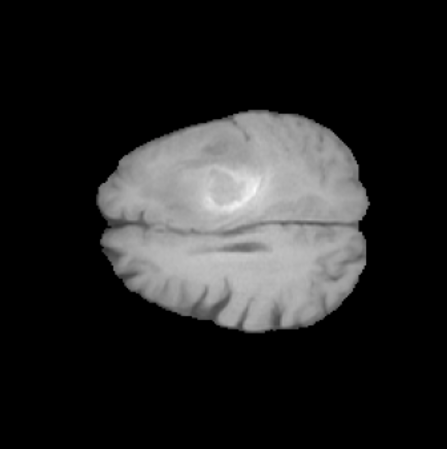
\includegraphics[width=0.4\textwidth]{./Images/Chapter2/t1.png}
          \captionsetup{hypcap=false}
          \captionof{figure}{Example of T1-weighted MRI sequence.}
          \label{fig:t1}
        \end{minipage}
        \vspace{\baselineskip}

  \item \textbf{T1 with contrast enhancement (T1ce)}: After gadolinium administration, areas with disrupted blood-brain barrier (characteristic of high-grade tumors) enhance, appearing hyperintense and revealing the active tumor core.

        \begin{minipage}{\linewidth}
          \centering
          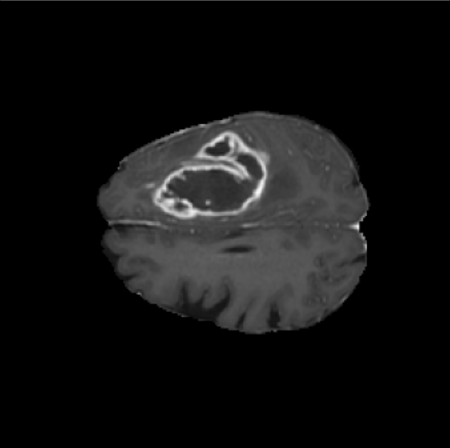
\includegraphics[width=0.4\textwidth]{./Images/Chapter2/t1ce.png}
          \captionsetup{hypcap=false}
          \captionof{figure}{Example of T1-weighted contrast-enhanced MRI sequence.}
          \label{fig:t1ce}
        \end{minipage}
        \vspace{\baselineskip}

  \item \textbf{T2-weighted (T2)}: Highlights areas with increased water content, making it valuable for identifying edema and infiltrative tumor components. Tumors and surrounding edema appear hyperintense.

        \begin{minipage}{\linewidth}
          \centering
          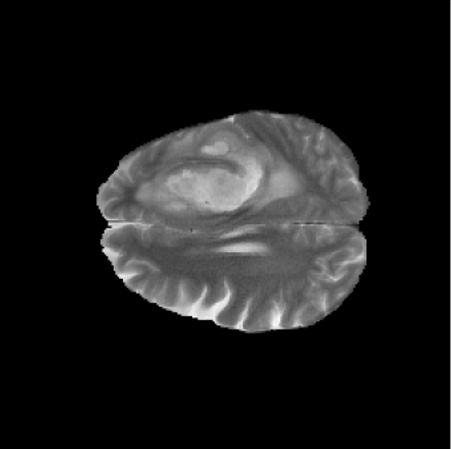
\includegraphics[width=0.4\textwidth]{./Images/Chapter2/t2.png}
          \captionsetup{hypcap=false}
          \captionof{figure}{Example of T2-weighted MRI sequence.}
          \label{fig:t2}
        \end{minipage}
        \vspace{\baselineskip}

  \item \textbf{Fluid-Attenuated Inversion Recovery (FLAIR)}: Suppresses cerebrospinal fluid signals, enhancing the visibility of periventricular lesions and edema associated with tumors.

        \begin{minipage}{\linewidth}
          \centering
          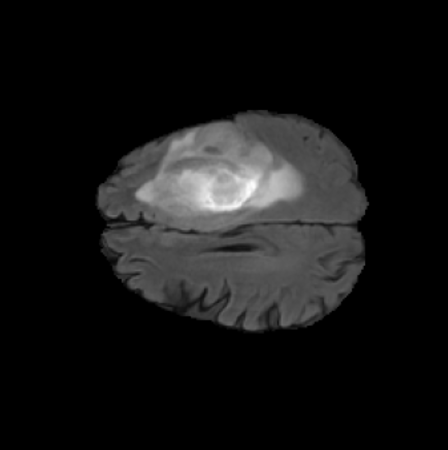
\includegraphics[width=0.4\textwidth]{./Images/Chapter2/flair.png}
          \captionsetup{hypcap=false}
          \captionof{figure}{Example of FLAIR MRI sequence.}
          \label{fig:t2-flair}
        \end{minipage}
        \vspace{\baselineskip}
\end{itemize}


Traditionally, neuroradiologists diagnose brain tumors by visually inspecting these multiple MRI sequences, mentally integrating information across modalities to determine tumor boundaries, assess grade, and identify critical structures \cite{DeAngelis2001}. This process is inherently subjective, time-consuming, and susceptible to inter-observer variability, with studies reporting considerable disagreement even among experienced radiologists  These limitations have driven significant interest in developing computational approaches for automated and semi-automated tumor analysis.

\section{The BraTS Dataset}

The Brain Tumor Segmentation (BraTS) challenge and dataset represent a landmark initiative in standardizing the evaluation of brain tumor segmentation algorithms \cite{Menze2015, Bakas2018}. Since its inception in 2012, BraTS has evolved into the most widely adopted benchmark for algorithm development and performance assessment in this domain \cite{Bakas2019}.

The BraTS dataset is particularly valuable due to its:

\begin{itemize}
  \item \textbf{Multimodal approach}: Each case includes four co-registered MRI sequences (T1, T1ce, T2, and FLAIR), enabling algorithms to leverage complementary information \cite{Bakas2017}.
  \item \textbf{Standardized preprocessing}: All images undergo skull-stripping, resampling to isotropic 1mm³ voxels, and registration to a common anatomical template, reducing technical variability \cite{Bakas2018}.
  \item \textbf{Expert annotations}: Each tumor is manually segmented by experienced neuroradiologists following a standardized protocol, with additional verification to ensure quality \cite{Menze2015}.
  \item \textbf{Multi-institutional data}: Images are acquired from multiple institutions using different scanners and protocols, promoting the development of robust algorithms \cite{Bakas2019}.
\end{itemize}

The BraTS 2020 dataset, specifically, comprises 369 training cases and 125 validation cases, with each case including pixel-wise annotations for three tumor sub-regions \cite{Bakas2020}:
\begin{enumerate}
  \item \textbf{Enhancing Tumor (ET)}: Areas showing hyperintensity in T1ce relative to T1
  \item \textbf{Tumor Core (TC)}: Encompassing the ET, necrotic components, and non-enhancing tumor
  \item \textbf{Whole Tumor (WT)}: Including all tumor tissues and surrounding edema
\end{enumerate}

This hierarchical annotation structure enables the evaluation of algorithms at multiple levels of detail, from gross tumor detection to fine-grained sub-region delineation \cite{Bakas2018}. The BraTS datasets and associated challenges have catalyzed significant methodological advances, with performance metrics improving consistently year over year \cite{Isensee2021}.

\section{Traditional Machine Learning Approaches}

Before the deep learning revolution, brain tumor segmentation and classification relied heavily on traditional machine learning techniques coupled with handcrafted feature extraction \cite{Gordillo2013}. These approaches typically followed a pipeline of preprocessing, feature extraction, and classification using conventional machine learning algorithms.

Support Vector Machines (SVMs) were particularly popular for brain tumor classification and segmentation due to their strong theoretical foundations and effectiveness with high-dimensional data \cite{Bauer2011}. Zacharaki et al.\ \cite{Zacharaki2009} developed an SVM-based system that extracted 161 features including intensity, texture, and shape characteristics from multi-parametric MRI, achieving 85\% accuracy in discriminating between different tumor types. Similarly, Reza and Iftekharuddin \cite{Reza2013} combined texture features with fractal analysis and SVM classification to segment brain tumors, demonstrating competitive performance on earlier BraTS datasets.

Random Forest (RF) classifiers also showed promise due to their robustness to overfitting and ability to handle multi-class problems efficiently. Zikic et al.\ \cite{Zikic2012} employed RF with context-aware features for brain tumor segmentation, while Festa et al.\ \cite{Festa2013} achieved strong results in the BraTS 2013 challenge using RF with handcrafted features. Tustison et al.\ \cite{Tustison2015} further refined this approach by incorporating an extensive feature set derived from multiple MRI sequences, winning the BraTS 2013 challenge.

K-Nearest Neighbors (k-NN) algorithms were explored by Simi and Joseph \cite{Simi2014}, who combined texture features with k-NN classification for tumor segmentation. Huang et al.\ \cite{Huang2014} also investigated k-NN for brain tumor classification using multispectral MRI features.

Despite their success, these traditional approaches faced significant limitations:

\begin{itemize}
  \item \textbf{Dependence on handcrafted features}: Their performance was heavily contingent on the quality of manually designed features, requiring substantial domain expertise \cite{Pandit2019}.
  \item \textbf{Limited contextual understanding}: Most methods struggled to incorporate broader spatial context, often relying on voxel-wise or small-patch features \cite{Havaei2017}.
  \item \textbf{Computational inefficiency}: Sequential processing of feature extraction followed by classification led to lengthy processing times impractical for clinical settings \cite{Sompong2017}.
  \item \textbf{Suboptimal performance on heterogeneous tumors}: The high variability in tumor appearance often challenged these methods, particularly for complex or atypical cases \cite{Menze2015}.
\end{itemize}

These limitations ultimately paved the way for the adoption of deep learning techniques, which could learn hierarchical features directly from data and better capture the complex patterns present in brain tumor images.

\section{Deep Learning in Brain Tumor Segmentation}

The advent of deep learning, particularly Convolutional Neural Networks (CNNs), has revolutionized brain tumor segmentation by enabling automatic hierarchical feature learning directly from imaging data \cite{Havaei2017}. This paradigm shift has eliminated the need for handcrafted features, dramatically improving segmentation accuracy and robustness.

Among deep learning architectures, U-Net has emerged as the cornerstone for medical image segmentation, including brain tumor analysis \cite{Ronneberger2015}. Its distinctive encoder-decoder structure with skip connections effectively combines localization and contextual information, preserving fine details while capturing broader tumor patterns. Urban et al.\ \cite{Urban2014} were among the first to apply CNNs to brain tumor segmentation, while Pereira et al.\ \cite{Pereira2016} demonstrated that carefully designed CNN architectures could outperform traditional methods on the BraTS challenge.

Several U-Net variants have been developed specifically for brain tumor segmentation:

\begin{itemize}
  \item \textbf{3D U-Net}: Çiçek et al.\ \cite{Cicek2016} extended the original 2D architecture to process volumetric data, better capturing the three-dimensional nature of tumors. Isensee et al.\ \cite{Isensee2018} further refined this approach, achieving top ranking in the BraTS 2018 challenge with a 3D U-Net variant.

  \item \textbf{U-Net++}: Zhou et al.\ \cite{Zhou2019} proposed a nested architecture with redesigned skip pathways to bridge the semantic gap between encoder and decoder features. Experimental results showed improved performance on several medical segmentation tasks, including brain tumors.

  \item \textbf{Attention U-Net}: Oktay et al.\ \cite{Oktay2018} incorporated attention gates to highlight relevant features and suppress irrelevant regions, improving segmentation accuracy particularly at tumor boundaries. Schlemper et al.\ \cite{Schlemper2019} demonstrated the effectiveness of this approach for multi-class tumor segmentation.
\end{itemize}

The performance of these deep learning models on BraTS challenges has improved consistently over time. In BraTS 2018, Myronenko \cite{Myronenko2018} achieved exceptional results with an encoder-decoder architecture incorporating variational components. McKinley et al.\ \cite{McKinley2019} further advanced the field with an ensemble of 3D U-Nets, achieving Dice scores of 0.91, 0.83, and 0.78 for whole tumor, tumor core, and enhancing tumor, respectively. The BraTS 2020 challenge saw even more impressive results, with top-performing methods consistently achieving Dice scores above 0.90 for whole tumor segmentation \cite{Isensee2021}.

The success of deep learning approaches for brain tumor segmentation can be attributed to several factors:

\begin{itemize}
  \item \textbf{End-to-end training}: These models learn optimal features directly from data rather than relying on predetermined feature extractors \cite{Havaei2017}.
  \item \textbf{Hierarchical feature representation}: The multiple convolutional layers capture features at various scales, from fine textures to global tumor shape \cite{Kamnitsas2017}.
  \item \textbf{Data augmentation techniques}: Strategies like random rotations, flipping, and elastic deformations effectively expand the training data, improving generalization \cite{Pereira2016}.
  \item \textbf{Ensemble approaches}: Combining multiple models or architectures has proven particularly effective, mitigating individual model weaknesses \cite{Wang2019}.
\end{itemize}

Despite these advancements, challenges remain in achieving clinically acceptable performance across diverse patient populations and imaging protocols, driving continuous innovation in the field.

\section{Tumor Classification Using Deep Features}

While segmentation delineates tumor boundaries, classification determines tumor type and characteristics—a critical aspect of diagnosis and treatment planning. Modern approaches increasingly leverage deep features, either independently or in conjunction with traditional machine learning classifiers like Support Vector Machines (SVMs).

Pretrained Convolutional Neural Networks (CNNs) have proven extremely effective as feature extractors for brain tumor classification. Afshar et al.\ \cite{Afshar2019} employed a modified ResNet architecture to extract deep features from brain MRI, achieving 93.68\% accuracy in classifying tumors into different grades. Similarly, Deepak and Ameer \cite{Deepak2019} utilized DenseNet for feature extraction followed by SVM classification, reporting improved performance compared to traditional methods. Sajjad et al.\ \cite{Sajjad2019} extended this approach by fine-tuning VGG-19 on brain tumor images, extracting features from intermediate layers for subsequent classification.

The integration of SVMs with deep features represents a particularly successful hybrid approach. Talo et al.\ \cite{Talo2019} extracted features from ResNet-50 and classified them using SVMs with different kernel functions, achieving 97.2\% accuracy in discriminating between tumor types. Cheng et al.\ \cite{Cheng2015} combined hand-crafted and deep features with SVM classification, demonstrating superior performance over either feature type alone. Kumar et al.\ \cite{Kumar2019} further refined this methodology by incorporating feature selection techniques before SVM classification, reducing dimensionality while maintaining discriminative power.

Convolutional Autoencoders (CAEs) offer an alternative approach to feature learning, particularly valuable when labeled data is scarce. Nalepa et al.\ \cite{Nalepa2019} employed a CAE to learn unsupervised representations from brain MRI, using these features with an SVM classifier for tumor grading. Khawaldeh et al.\ \cite{Khawaldeh2018} similarly used CAEs for feature extraction followed by a non-linear SVM, achieving 91.2\% classification accuracy. Sun et al.\ \cite{Sun2018} combined CAE-derived features with a random forest classifier, demonstrating robust performance even with limited training examples.

Feature fusion techniques have emerged as a powerful strategy to combine complementary information. Amin et al.\ \cite{Amin2020} developed a multi-modal fusion approach combining features from different MRI sequences, improving classification accuracy by 4-6\% compared to single-modality methods. Zhou et al.\ \cite{Zhou2020} proposed a hierarchical feature fusion framework integrating both low-level and high-level features from multiple CNN layers, achieving 96.7\% accuracy in glioma grading. Yang et al.\ \cite{Yang2018} introduced a multi-stream architecture extracting and fusing features from different MRI modalities, demonstrating superior performance over single-stream networks.

The success of these deep feature-based approaches stems from their ability to:
\begin{itemize}
  \item Capture complex, high-level tumor characteristics not easily described by handcrafted features \cite{Afshar2019}
  \item Leverage transfer learning from models pre-trained on large datasets \cite{Sajjad2019}
  \item Combine the representational power of deep learning with the strong theoretical foundations of classical classifiers like SVM \cite{Talo2019}
\end{itemize}

The integration of deep features with traditional classifiers represents a bridge between conventional and modern approaches, often yielding superior performance compared to either method used in isolation.

\section{Multiclass Tumor Region Segmentation}

Accurate delineation of different tumor sub-regions represents one of the most challenging aspects of brain tumor analysis, requiring discrimination between biologically distinct components that may appear visually similar \cite{Bakas2018}. The BraTS challenge specifically evaluates algorithms on their ability to segment three tumor sub-components: Enhancing Tumor (ET), Tumor Core (TC), and Whole Tumor (WT).

Multi-class tumor segmentation approaches have evolved significantly in recent years. Zhao et al.\ \cite{Zhao2018} proposed a multi-scale CNN architecture specifically designed to address the hierarchical nature of tumor sub-regions, achieving meaningful improvements in enhancing tumor segmentation. Wang et al.\ \cite{Wang2017} developed a cascaded approach where initial whole tumor segmentation guided subsequent sub-region delineation, reducing false positives in non-tumor regions. Kamnitsas et al.\ \cite{Kamnitsas2017} introduced DeepMedic, a dual-pathway 3D CNN architecture that simultaneously processed input at different resolutions, effectively capturing both fine details and broader contextual information.

Several specific challenges complicate multi-class tumor segmentation:

\begin{itemize}
  \item \textbf{Data imbalance}: Tumor sub-regions occupy a small fraction of the brain volume, creating severe class imbalance. Myronenko \cite{Myronenko2018} addressed this through a combination of weighted loss functions and focal loss, specifically targeting challenging boundary regions. Isensee et al.\ \cite{Isensee2018} employed a region-based training strategy that oversampled patches containing tumor sub-regions, achieving more balanced training.

  \item \textbf{Overlapping regions}: The hierarchical nature of tumor sub-regions (ET $\subset$ TC $\subset$ WT) creates inherent overlap that can confuse classification systems. McKinley et al.\ \cite{McKinley2019} tackled this through a cascaded architecture with hierarchical loss functions that explicitly modeled these relationships. Jiang et al.\ \cite{Jiang2020} proposed a multi-task learning framework where auxiliary tasks helped distinguish overlapping regions.

  \item \textbf{Variable appearance}: Tumor sub-regions show considerable variability across patients and can mimic other pathologies. Zhou et al.\ \cite{Zhou2020} employed attention mechanisms to focus on discriminative features for each sub-region, while Wang et al.\ \cite{Wang2019} leveraged ensemble techniques to improve robustness to appearance variations.

  \item \textbf{Need for multi-modal integration}: Different tumor sub-regions are best visualized in specific MRI sequences (e.g., enhancing tumor in T1ce, edema in FLAIR). Shen et al.\ \cite{Shen2019} developed multi-encoder architectures that extracted sequence-specific features before fusion, while Chen et al.\ \cite{Chen2019} employed attention-based fusion to weight the contribution of each modality dynamically.
\end{itemize}

Performance metrics for multi-class segmentation vary considerably across sub-regions. While whole tumor segmentation typically achieves Dice scores around 0.90 in recent BraTS challenges, enhancing tumor segmentation remains more challenging with top performances around 0.80-0.85 \cite{Bakas2020}. This performance gap reflects the smaller size and more variable appearance of enhancing components compared to the whole tumor region.

Recent work has increasingly focused on uncertainty estimation in multi-class segmentation. Mehta et al.\ \cite{Mehta2020} incorporated Bayesian neural networks to provide uncertainty maps alongside segmentations, highlighting regions where the model lacked confidence. Eaton-Rosen et al.\ \cite{EatonRosen2018} similarly demonstrated the value of uncertainty quantification for clinical decision support, particularly for ambiguous tumor boundaries.

The continued advancement of multi-class tumor segmentation approaches promises to improve diagnostic accuracy and treatment planning by providing more detailed characterization of tumor heterogeneity.

\section{Challenges in the Field}

Despite significant progress, several persistent challenges continue to impact the development and clinical translation of automated brain tumor analysis systems.

\textbf{Class imbalance} remains a fundamental issue in both segmentation and classification tasks. Brain tumors typically occupy less than 1\% of the total brain volume, creating extreme imbalance that can bias models toward the majority (healthy tissue) class \cite{Pereira2016}. While techniques such as patch-based training \cite{Havaei2017}, specialized loss functions \cite{Isensee2018}, and data augmentation \cite{Wang2019} have partially addressed this issue, performance on smaller tumor sub-regions (particularly enhancing tumor) continues to lag behind whole tumor segmentation.

The \textbf{interpretability of deep models} presents another significant hurdle, particularly for clinical adoption. The "black box" nature of deep learning approaches creates reluctance among clinicians to trust automated segmentations without understanding the underlying decision process \cite{Holzinger2017}. Recent work by Natekar et al.\ \cite{Natekar2020} has explored visualization techniques to highlight features influencing segmentation decisions, while Lucieri et al.\ \cite{Lucieri2020} demonstrated the value of attention maps for explaining tumor classification outcomes. Despite these efforts, creating truly interpretable deep learning systems remains an open challenge.

\textbf{Generalization across different MRI scanners and patients} continues to limit clinical applicability. Models trained on specific datasets often experience performance degradation when applied to images acquired with different hardware, field strengths, or acquisition parameters \cite{Menze2015}. Zech et al.\ \cite{Zech2018} documented this domain shift problem in medical imaging, while Kamnitsas et al.\ \cite{Kamnitsas2017} proposed domain adaptation techniques to mitigate its effects. More recently, Shaw et al.\ \cite{Shaw2020} explored adversarial domain adaptation specifically for brain tumor segmentation, showing promising results in cross-scanner generalization.

The \textbf{lack of labeled data} remains a fundamental limitation, particularly for rare tumor types or unusual presentations. While the BraTS dataset has grown substantially, it still represents a fraction of the true biological variability of brain tumors \cite{Bakas2019}. Semi-supervised approaches by Sedai et al.\ \cite{Sedai2019} leverage unlabeled data to improve generalization, while Zhao et al.\ \cite{Zhao2019b} demonstrated promising results with data-efficient few-shot learning techniques. Transfer learning approaches by Ghafoorian et al.\ \cite{Ghafoorian2017} have also shown potential in adapting pre-trained models to limited target datasets.

Additional challenges include:

\begin{itemize}
  \item \textbf{Computational efficiency}: 3D deep learning models often require substantial computational resources beyond what's available in many clinical settings \cite{Kamnitsas2017}.
  \item \textbf{Longitudinal analysis}: Most current approaches treat each time point independently, missing the opportunity to leverage temporal information in patient monitoring \cite{Weninger2018}.
  \item \textbf{Integration with other data types}: Combining imaging with clinical, genomic, and pathological data remains challenging despite its potential to improve diagnostic accuracy \cite{Bakas2019}.
  \item \textbf{Clinically relevant evaluation metrics}: Standard technical metrics like Dice coefficients may not directly translate to clinical utility, creating a disconnect between research advances and clinical impact \cite{MaierHein2018}.
\end{itemize}

Addressing these challenges will require multidisciplinary collaboration between computer scientists, medical imaging experts, and clinicians to develop solutions that are not only technically sophisticated but also clinically relevant and practically deployable.
